% !TEX program = xelatex
\documentclass[oneside]{article}

\title{%
\textbf{Vintage Rent}  \\
\large Documentatie \\
(Programare Avansata pe Obiecte)}
\date{}
\author{Dinu Florin-Silviu \\ grupa 231}

\makeatletter
\renewcommand{\@seccntformat}[1]{}
\makeatother

\usepackage{tikz}
\usepackage{forest}
\usepackage{hyperref}
\usepackage{amsthm}
\usepackage{amssymb}
\usepackage[romanian]{babel}
\usepackage[a4paper, margin=3cm]{geometry}
\usepackage{enumitem}
\usepackage{listings}
\usepackage{fontspec}
\usepackage{xcolor}
\usepackage{textcomp}
\usepackage{graphicx}
\usepackage{tabularx}
\usepackage{titlesec}
\usepackage{mathtools}
\usepackage{bookmark}
\usepackage{lmodern}

\graphicspath{ {./img/} }

\lstset{
%  tabsize=4,
extendedchars=true,
        % %upquote=false,
        % aboveskip=\baselineskip,
        columns=fixed,
        showstringspaces=false,
        extendedchars=true,
        breaklines=true,
        % prebreak = \raisebox{0ex}[0ex][0ex]{\ensuremath{\hookleftarrow}},
        showtabs=false,
        showspaces=false,
        identifierstyle=\ttfamily,
        % keywordstyle=\color[rgb]{0,0,1},
        % commentstyle=\color[rgb]{0.133,0.545,0.133},
        % stringstyle=\color[rgb]{0.627,0.126,0.941},
        % language=SQL
        frame=lines,
        literate=%
    {€}{\euro}1%
    {§}{\S}1%
    {°}{\textdegree{}}1%
    {ä}{{\"a}}1%
    {ö}{{\"o}}1%
    {ü}{{\"u}}1%
    {ß}{{\ss}}1%
    {Ä}{{\"A}}1%
    {Ö}{{\"O}}1%
    {Ü}{{\"U}}1%
    {µ}{\textmu}1%
    {¹}{{\textsuperscript{1}}}1%
    {²}{{\textsuperscript{2}}}1%
    {³}{{\textsuperscript{3}}}1%
    {¼}{\textonequarter}1%
    {½}{\textonehalf}1%
    {¢}{\textcent}1%
}


\begin{document}
\pagenumbering{gobble}
\maketitle
\tableofcontents

\newpage
\pagenumbering{arabic}

\section[Introducere]{Introducere}
\paragraph{} Aplicatia permite gestionarea unui magazin care inchiriaza camere vintage. Avem utilizatori care pot fi angajati, clienti sau administratori de site. Acestora le sunt puse la dispozitie camere de diverse tipuri si obiective. Ei pot alege sa inchirieze oricare pereche de camera si obiectiv doresc. Daca apar probleme, angajatii pot adauga penalizari inchirierii.

\paragraph{}Ca o prima idee despre ce si cum se poate face, atasez diagrama relationala a bazei de date. Proiectul a fost gandit pentru un anumit workflow care este implementat si in aplicatia Java.

\begin{figure}[ht]
    \centering
    \noindent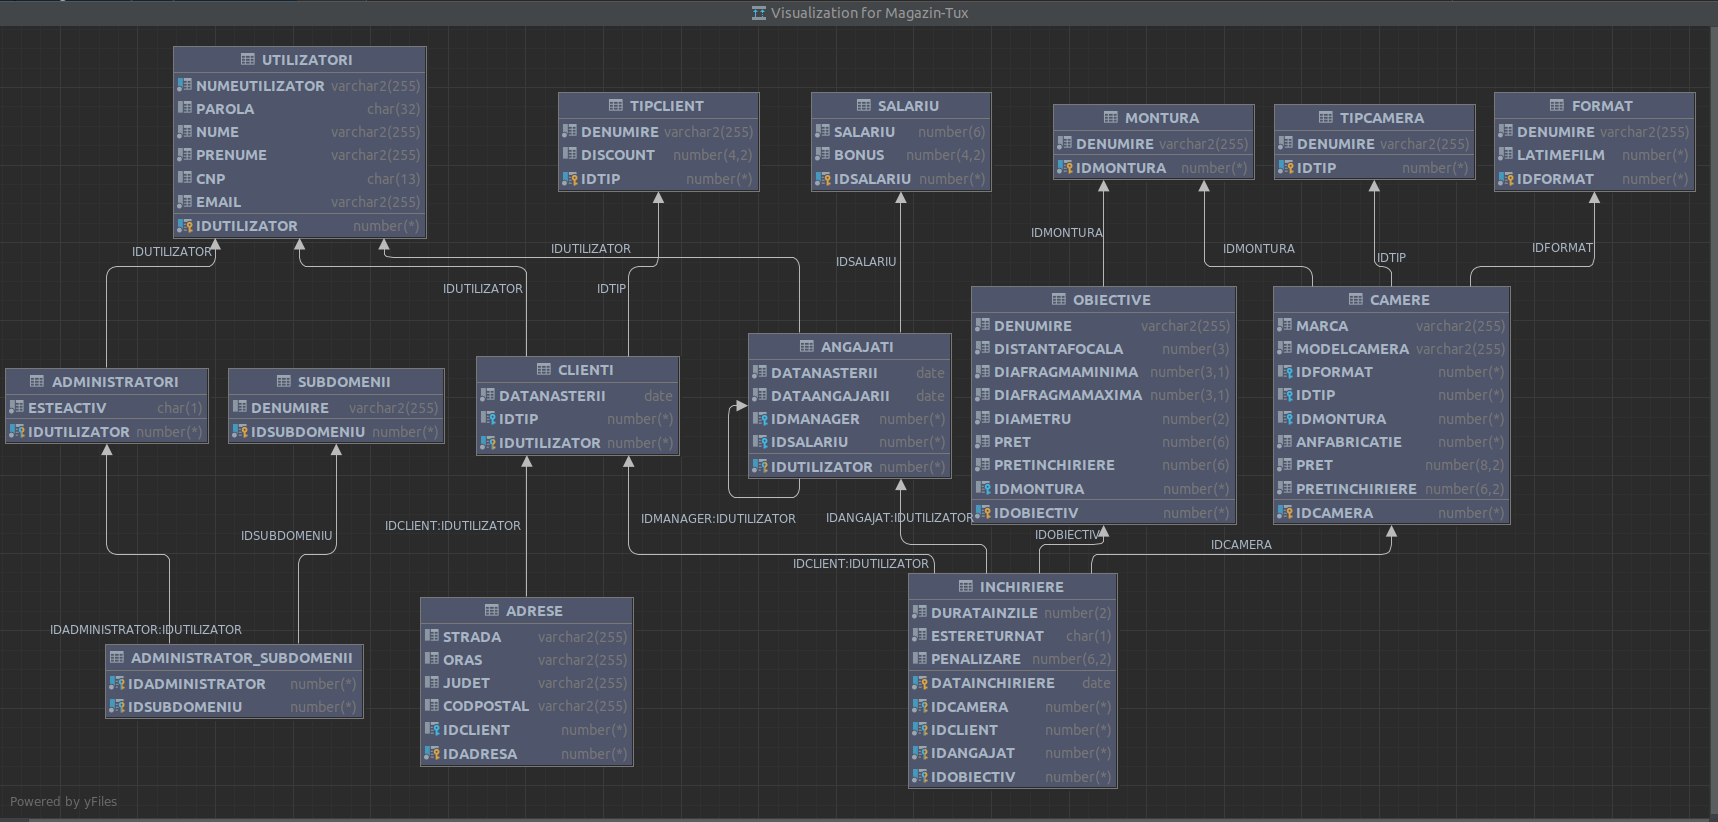
\includegraphics[width=\linewidth]{diagrama.png}
    \caption{Diagrama relationala}
    \label{fig:diagrama}
\end{figure}

\section[Main]{Main}
\paragraph{}Entry pointul in program se afla in \textbf{org.vintage.Main}, metoda \textbf{main}. Mai intai se initializeaza tema pentru GUI, apoi se porneste serviciul de audit \textbf{CsvLogger}. Apoi din main se lanseaza un thread separat si se asteapta sa se faca joinul. Acest lucru ne permite sa detectam cand programul este inchis si sa logam aceasta operatie. 
\paragraph{} Threadul deschis de main incepe prin a afisa splash screenul. In timpul afisarii se deschide un thread nou pentru conectarea la \textbf{baza de date Oracle} si se verifica fisierele \textbf{csv} pentru a avea putea fi procesate de al doilea tip de datasource. Atributul atomic boolean \textbf{isOracleUp} tine cont daca s-a putut realiza conexiunea la baza de date. Daca aceasta s-a realizat, atunci se va folosi default baza de date, daca nu, atunci se va folosi default csvul. Datasourceul poate fi schimbat in timpul rularii programului din meniul corespunzator, deci in aceasta etapa doar definim defaulturile.
\paragraph{} Dupa ce threadul care face conexiunile se termina, se rezuma threadul \textbf{tmain} care va face dispose splash screenului dupa minim 3 secunde (in total cu timpul de conectare la data sourceuri). Apoi se incepe cu MainGUI care reprezinta interfata grafica principala.

\section[GUI]{GUI}
\subsection[MainGUI]{MainGUI}
\paragraph{}
\begin{figure}[ht]
    \centering
    \noindent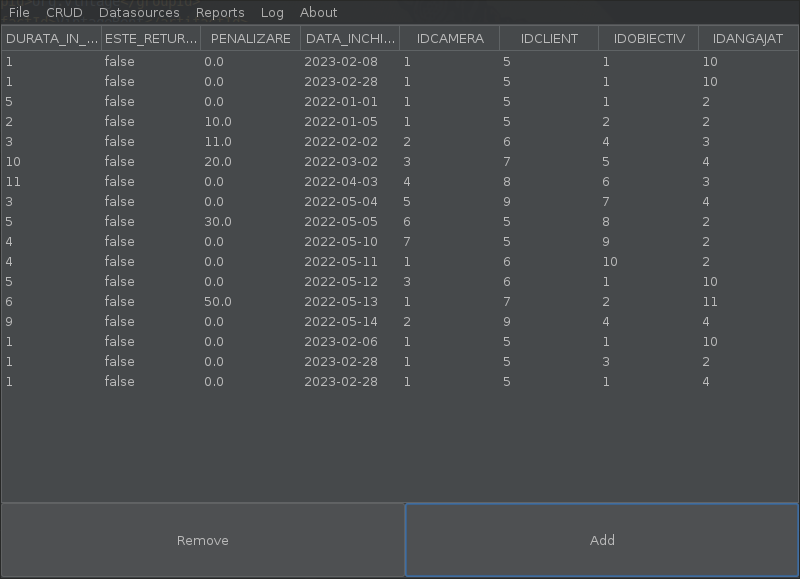
\includegraphics[scale=0.4]{program.png}
    \caption{Main GUI}
    \label{fig:maingui}
\end{figure}

Pentru tema am folosit \textbf{com.formdev.flatlaf} si am initializat \textbf{FlatDarkLaf}. Mai jos este codul dependentei din \textbf{pom.xml}.
\begin{center}
    \begin{lstlisting}
    <dependency>
        <groupId>com.formdev</groupId>
        <artifactId>flatlaf</artifactId>
        <version>3.0</version>
    </dependency>
    \end{lstlisting}
\end{center}

\paragraph{} Interfata grafica principala consta dintr-o \textbf{bara de meniu} si un \textbf{gridbaglayout} in care este pus un \textbf{JTable} si doua butoane de \textbf{remove} si \textbf{add}.

\paragraph{Bara de meniu} are mai multe elemente:
\begin{enumerate}
    \item File - de aici se poate iesi din program
    \item CRUD - contine tabelele pe care se poate lucra si se va face update la alegerea oricarui tabel, evident ca folosind datele din data sourceul selectat
    \item Datasources - contine sursele de date disponibile si se va face update la alegerea oricarei surse de date
    \item Rapoarte - contine rapoartele
    \item Log - contine un item pentru afisarea logurilor
    \item About - afiseaza informatii despre program
\end{enumerate}

\paragraph{JTable} este evident continut intr-un \textbf{JScrollPane} si are un data source dat prima data de \textbf{Rent} pentru \textbf{read}. Contine un eveniment de setare a valorii in caz de \textbf{update}. Unele tabele pot fi sortate, altele nu, depinde de la caz la caz. Oricum, chiar si in cele care pot fi  sortate, operatiunile decurg normal, deoarece se obtine indexul corect al liniei si coloanei.

\paragraph{Butonul remove} va sterge randul selectat atunci cand este apasat.

\paragraph{Butonul add} va deschide o fereastra personalizata in functie de fiecare tabela in parte. In continuare voi vorbi despre ferestrele de adaugare.

\subsection[Add]{Add}
\begin{figure}[ht]
    \centering
    \noindent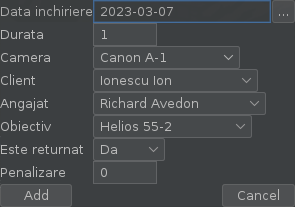
\includegraphics[scale=0.7]{addgui.png}
    \caption{Add GUI}
    \label{fig:addgui}
\end{figure}

\paragraph{} Ferestrele de adaugare sunt facute in functie de fiecare clasa in parte. Ca element comun toate contin un \textbf{gridbaglayout}, un buton de adaugare si unul de iesire, precum si mai multe JLable-uri.

\paragraph{} Elementele optionale pe care le pot contine sunt:
\begin{enumerate}
    \item \textbf{JTextField} pentru text normal
    \item \textbf{JComboBox} in cazul unei chei externe pentru alegerea in functie de informatiile din tabelul de legatura
    \item \textbf{JDatePickerImpl} pentru alegerea datelor calendaristice
\end{enumerate}

\paragraph{} Daca primul este evident, pentru celelalte doua voi detalia.

\paragraph{JComboBox} reprezinta un combo box pentru a alege datele in functie de ce se afla in tabelul de legatura. Ca element, am creat \textbf{org.gui.custom.ComboItem} pentru a putea opera cu o cheie si o valoare. Cheia reprezinta valoarea campului de legatura, iar valoarea ceea ce se va afisa.

\paragraph{JDatePickerImpl} reprezinta un date picker de la \textbf{org.jdatepicker.jdatepicker}. Acesta poate vine cu un panou care se afiseaza dinamic pentru alegerea datei calendaristice. Codul pentru dependenta adaugat in \textbf{pom.xml} este:
\begin{center}
    \begin{lstlisting}
<dependency>
    <groupId>org.jdatepicker</groupId>
    <artifactId>jdatepicker</artifactId>
    <version>1.3.4</version>
</dependency>
    \end{lstlisting}
\end{center}

\subsection[Rapoarte]{Rapoarte}
\paragraph{Raport clienti} reprezinta raportul in care se pot afisa date despre ce a inchiriat un client. Acesta contine un \textbf{JComboBox} pentru a alege clientul cu un eveniment de schimbare astfel incat sa se actualizeze automat datele din \textbf{JTable}-ul de mai jos. De asemenea, contine si un buton de exit.


\subsection[Log]{Log}
\begin{figure}[ht]
    \centering
    \noindent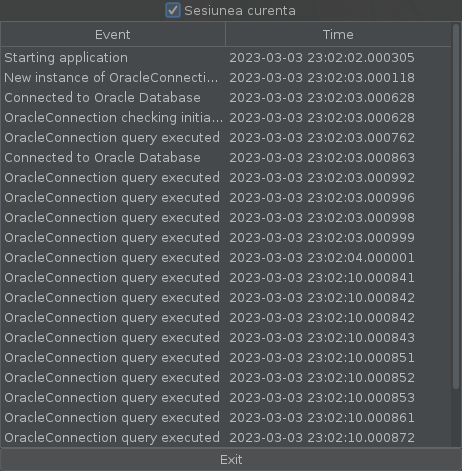
\includegraphics[scale=0.6]{loggui.png}
    \caption{Log GUI}
    \label{fig:loggui}
\end{figure}
\paragraph{} Contine logurile sesiunii curente, dar si un \textbf{JCheckBox} astfel incat sa poata fi vazute toate. Acestea sunt scrise intr-un fisier CSV si preluate de acolo intr-un \textbf{JTable} continut intr-un \textbf{JScrollPane}.

\section[Conexiunea la data sourceuri]{Conexiunea la data sourceuri}

\section[Modele]{Modele}

\section[Serviciul de audit]{Serviciul de audit}
\paragraph{CsvLogger} este numele serviciului de audit care scrie logurile intr-un fisier csv. Acesta extinde \textbf{java.util.logging.Logger} si este de tip singleton. Are un constructor privat si singurul mod in care poate fi creata instanta este prin metoda statica \textbf{getInstance}.

\paragraph{Metoda de scriere} log primeste un mesaj de tip String si il scrie in fisier.

\paragraph{Metodele de citire} readLog() si readLogToday() citesc intreg fisierul de log, respectiv doar cel de la inceputul sesiunii si pana acum si corespund optiunilor din interfata grafica. Ambele returneaza un \textbf{Pair<List<String>, List<List<String>>>} cu headerul, respectiv corpul fisierului.

\section[Rapoarte]{Rapoarte}
\paragraph{} Rapoartele si alte actiuni pot fi accesate direct din \textbf{org.actions.MainService}.

\subsection[Raport client]{Raport client}
\paragraph{} Acesta primeste un intreg care reprezinta ID-ul clientului si un tip de baza de date. Returneaza un \textbf{Map<String, String>} reprezentand maparea tuturor datelor obtinute. Ca mentiune separata, pentru a numara camerele distincte am optat pentru o integrare comuna intre CSV si bazele de date, asa ca am efectuat o singura interogare si le pun intr-un \textbf{HashSet<Integer>}, iar apoi extrag dimensiunea lui.

\section[Clase ajutatoare]{Clase ajutatoare}
\subsection[Pair<T, U>]{Pair<T, U>}
\paragraph{} Deoarece in Java nu exista un tip pair nativ, am scris o clasa care foloseste doua templateuri, T si U, si creaza o pereche mapand obiectele pe atributele first si second. Acesta sunt publice, dar se pot accesa si prin getteri.

\section[Resurse]{Resurse}

\section[Alte mentiuni despre cod]{Alte mentiuni despre cod}

\section[Workflow GitHub]{Workflow GitHub}
\paragraph{} Actiunea de publicare a unei versiuni noi pe GitHub are urmatorii pasi:
\begin{enumerate}
    \item Checkout
    \item Setare Java 17 Oracle
    \item Preluarea versiunii proiectului cu ajutorul Maven din pom.xml
    \item Buildul facut de Maven
    \item Uploadul artefcatului de realease (fisierul .jar) in mediul actiunii
    \item Crearea pachetului de release
    \item Atasarea artefactului de release la pachet
\end{enumerate}

\paragraph{} Toate aceste lucruri se pot face atat manual cat si la fiecare push pe main. De aceea pentru fiecare versiune noua se va lucra pe un branch separat.

\paragraph{} Fisierul de workflow se afla in \textbf{./.github/workflows/main.yml}.

\end{document}